\section{Technical standards}
\label{sect:standards}
In this section we define explicitly the technical data exchange format for the
logical structures defined in the previous subsections.

%%%%%%%%%%%%%%%%%%%%%%%%%%%%%%%%%%%%%%%%%%%%%%%%%%%%%%%%%%%%%%%%%%%%%%%%%%%%%%%
\subsection{File encoding and data storage format per type}
Below we propose a JSON format \citep{ecma2013json} for exchanging data
validation reports.  Although it is a textual format, the JSON standard does
not impose restrictions on the encoding used. It is left explicitly to
standards built upon JSON to define an encoding \citep[pp ii]{ecma2013json}. In
this standard we follow the currently most widely applied standard (see
Figure~\ref{fig:encoding}) with the following demand.

\begin{center}
\captionof{table}{File encoding used for validation reports}
\label{tab:encoding}
\begin{tabular}{|p{0.97\textwidth}|}
\hline
Validation reports  are encoded in \code{UTF-8}.\\
\hline
\end{tabular}
\end{center}

\begin{figure}[t]
\centering
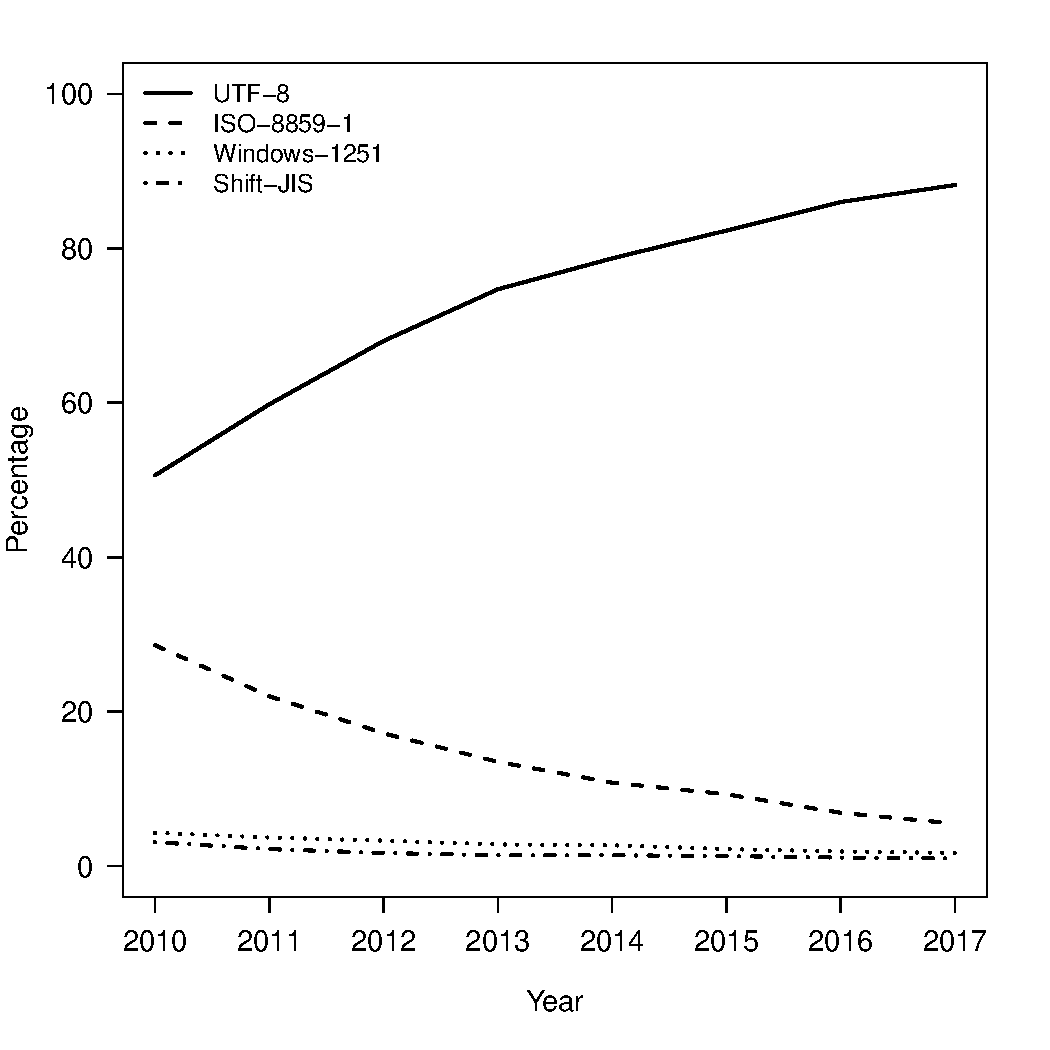
\includegraphics[width=0.7\textwidth]{fig/encoding_use.pdf}
\caption{Percentages of encoding standards used on the web \citep{w3techs2017}.}
\label{fig:encoding}
\end{figure}

The different data types within a file are to be formatted according to
commonly used standards where possible. In particular, data in validation
reports are encoded as stated in Table~\ref{tab:dataformat}.
\begin{center}
\captionof{table}{Format of data types in validation reports.}
\begin{tabular}{|lp{0.92\textwidth}|}
\hline
1&Numbers are encoded in a valid decimal ISO/IEC/IEEE 60559:2011 (IEEE 754) format
\citep{ieee:2008}. \\
2&Date-time data shall be denoted in ISO 8601 format \code{YYMMDDTHHmmss+HHMM} \citep{iso2004data}. \\
\hline
\end{tabular}
\label{tab:dataformat}
\end{center}





%%%%%%%%%%%%%%%%%%%%%%%%%%%%%%%%%%%%%%%%%%%%%%%%%%%%%%%%%%%%%%%%%%%%%%%%%%%%%%%
\subsection{JSON Schemas}
The JSON message consists of records that are either of type validation,
or aggregation. The former are schematically represented as follows
\begin{align*}
\textsf{validation}&:=\langle
  \textsf{id}
, \textsf{type}:=\code{"validation"}
, \textsf{event}
, \textsf{rule}
,\textsf{data}
,\textsf{value}\rangle\\
\textsf{event} &= \langle
  \textsf{time}
, \textsf{actor}
, agent
, trigger\rangle\\
\textsf{rule} &:=\langle
  \textsf{language}
, \textsf{expression}
, \textsf{severity}
, status\rangle\\
\textsf{data} &:=\langle
  \textsf{source}
, \textsf{target}
, description\rangle,
\end{align*}
where `id' is a unique identifier, `type' has a fixed value that labels the
object type and `value' is a validation result ($0$, $1$ or $\na{}$). In the
above scheme, the fields in $italics$ are optional. 

Objects of type type `aggregation' are schematically described as
\begin{align*}
\textsf{aggregation} &:=\langle
  \textsf{id}
, \textsf{type}=\code{"aggregation"}
, \textsf{event}
, \textsf{aggregate}
, \textsf{data}
,\textsf{value}\rangle\\
\textsf{event} &:= \langle
  \textsf{time}
, \textsf{actor}\rangle\\
\textsf{aggregate} &:=\langle
  \textsf{language}
, \textsf{expression}\rangle\\
\textsf{data} &:=\langle
  \textsf{source}
, \textsf{target}
, description\rangle,
\end{align*}
where `value' is the aggregate value, represented as a string.

These object types are translations of Definitions~\ref{def:validationresult},
\ref{def:confrontation} and \ref{def:aggregation}, with components derived from
the logical descriptions in \S\ref{sect:basicreportstructure}.

The JSON scheme defining these objects can be found in the listings on
pages~\pageref{lst:valrep1}--\pageref{lst:valrep3}. The full code can also be
found at github:
\begin{center}
\href{https://github.com/data-cleaning/ValidatReport}{https://github.com/data-cleaning/ValidatReport}
\end{center}
%
\lstinputlisting[frame=single
  , linewidth=1.15\textwidth
  , lastline=36
  , float=h,caption=JSON schema for a validation report.
  , label=lst:valrep1]{../json/validation_report.json}
%
%
\newpage



\lstinputlisting[frame=single
  , linewidth=1.15\textwidth
  , firstnumber=37
  , firstline=37
  , float=h,caption=JSON schema for a validation report---continued.
  , label=lst:valrep3]{../json/validation_report.json}

